\subsection{Model Linearization with Control System Toolbox}\label{app:linearization}
    % \dots\textit{explanation}\dots
    This appendix contains the step-by-step instructions to linearize the chosen SCARS model. In the case of this example, the aim is to acquire linear model of satellite with added actuators, to use it for control system design. The relevant block in this SCARS model are \textbf{Satellite Dynamics} as a core of simulation, one \textbf{Reaction Wheel (1-axis, X/Y/Z)} for each major axis. \autoref{fig:lin_model} presents the whole model used in this example.

    
    \begin{figure}[H]
        \centering
        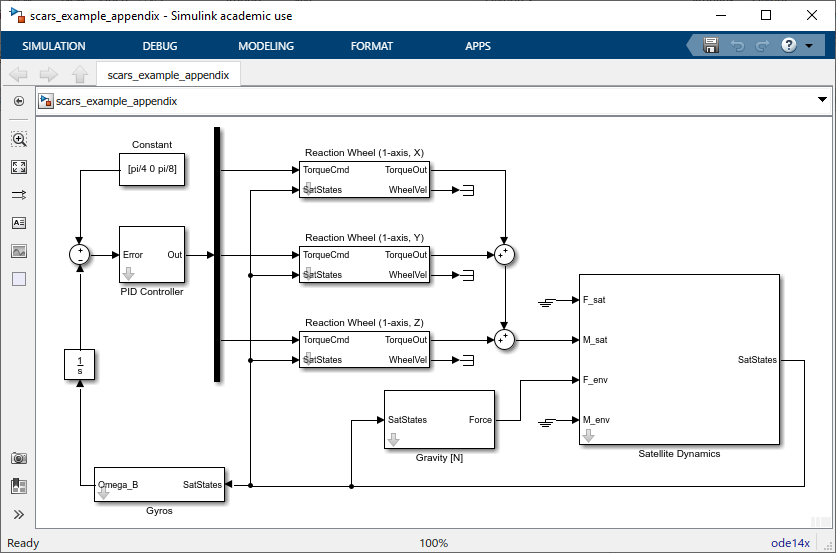
\includegraphics[width=1\textwidth]{appendix/lin_model.png}
        \caption{Satellite model built with SCARS for purposes of linearization presentation}
        \label{fig:lin_model}
    \end{figure}


        
    \subsubsection*{Step 1: Create output signals}

        To linearize the SCARS model one has to determine inputs and outputs which will be represented by the acquired linearized model. While the model inputs are same as the actuators blocks inputs (or \textbf{Demux} outputs), the outputs have to be extracted from \textbf{SatStates} bus. To do that, the user has to add \textbf{Bus Selector} block and choose, in case of this example, \textbf{Euler\_B} signal, as seen on \autoref{fig:lin_selector}. 
        
        It has to be noted that if any controller is set up to provide input signal, like \textbf{PID Controller} in this example, it has to be commented out from the model before linearization.

        \begin{figure}[H]
            \centering
            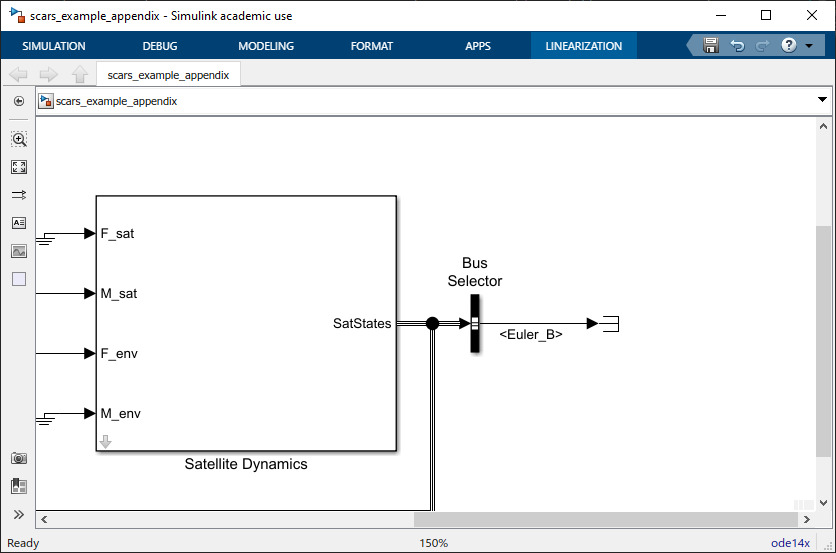
\includegraphics[width=1\textwidth]{appendix/bus_selector.png}
            \caption{Extraction of output signal from bus port}
            \label{fig:lin_selector}
        \end{figure}



    \subsubsection*{Step 2: Select input and output signals}

        Once all signals are available in the model, it is necessary to properly mark them for Simulink Linear Analysis Tool. To do that, the user has to open \textit{Linearization Manager} from \textit{Apps} tab in Simulink model editor. Then, a signal has to be chosen and in \textit{Linearization} tab a correct type of signal has to be applied. In case of input it has to be \textit{Open-loop Input}, as seen on \autoref{fig:lin_io} \subref{sub:lin_input}, and in case of output it has to be \textit{Open-loop Output}, as seen on \autoref{fig:lin_io} \subref{sub:lin_output}. Small arrow icons over the signal route show that the I/O ports are properly set up.

        \begin{figure}[H]
            \centering
            \subfloat[Open loop input setup]{{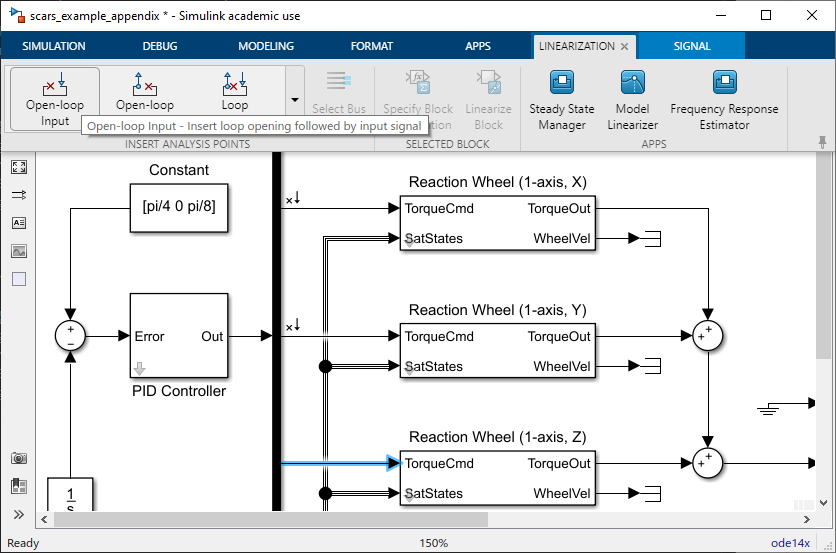
\includegraphics[width=1\textwidth]{appendix/input.png}\label{sub:lin_input} }}%
            % \qquad
            \\
            \subfloat[Open loop output setup]{{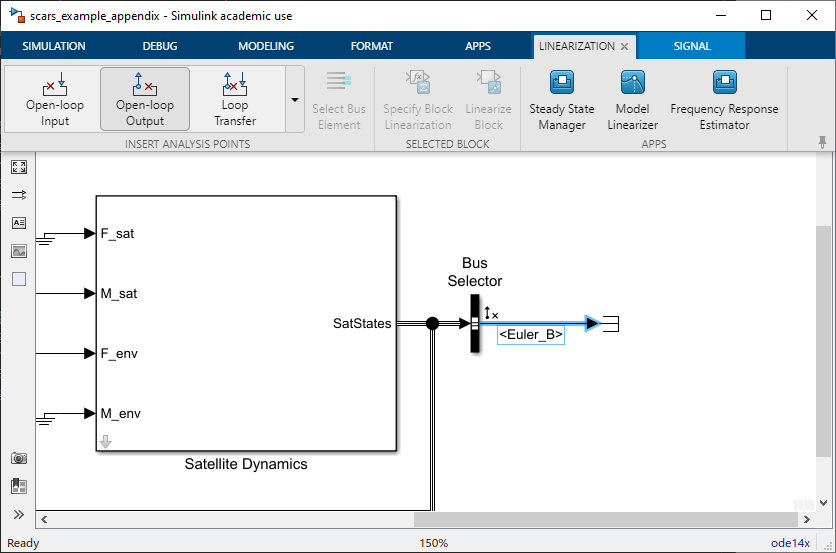
\includegraphics[width=1\textwidth]{appendix/output.png}\label{sub:lin_output} }}%
            \caption{Step 2: Open loop I/O setup}%
            \label{fig:lin_io}%
        \end{figure}

        

    \subsubsection*{Step 3: Trim the model}
        After setting up the model I/O signals, the user can open \textit{Linear Analysis Tool} by choosing \textit{Model Linearizer} from either \textit{Apps} or \textit{Linearization} tabs. Once loaded, the initial conditions have to be set up for the linearization process. To do that, the user can trim the model by choosing \textit{Trim Model...} from \textit{Model Initial Condition} in \textit{Setup} section of \textit{Linear Analysis} tab.
         
        For this example, the only checkboxes that need to be marked in opened dialog are \textit{Steady State} for all three states of both \verb|Satellite Dynamics/6DOF ECEF (Quaternion)/p,q,r| and \verb|Satellite Dynamics/Euler_B|, as can be seen on \autoref{fig:lin_trimming}. After that the user has to click the \textit{Start trimming} button.

        \begin{figure}[H]
            \centering
            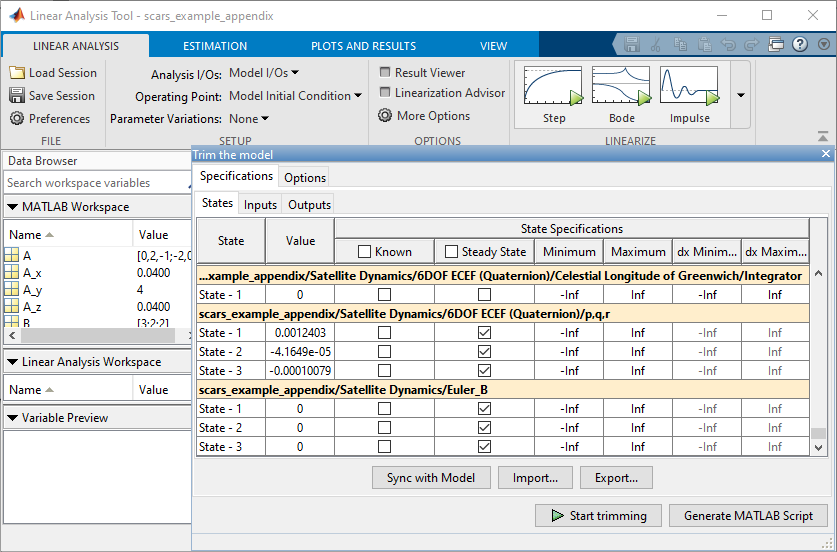
\includegraphics[width=1\textwidth]{appendix/trimming.png}
            \caption{Model trimming}
            \label{fig:lin_trimming}
        \end{figure}

        

    \subsubsection*{Step 4: Linearization of the model}
        Once the model has been trimmed the initial conditions are automatically set. Then, the user can launch linearization process from \textit{Linearize} section of \textit{Linear Analysis} tab, by choosing any plot or option there. This should result in a plot (if chosen) and linearized model available in \textit{Linear Analysis Workspace}, under the name \verb|linsys1| or similar. The user can then move it it \textit{MATLAB Workspace} and use it for various purposes, such as control system design as presented in example in \autoref{sec:control_design}.

        \begin{figure}[H]
            \centering
            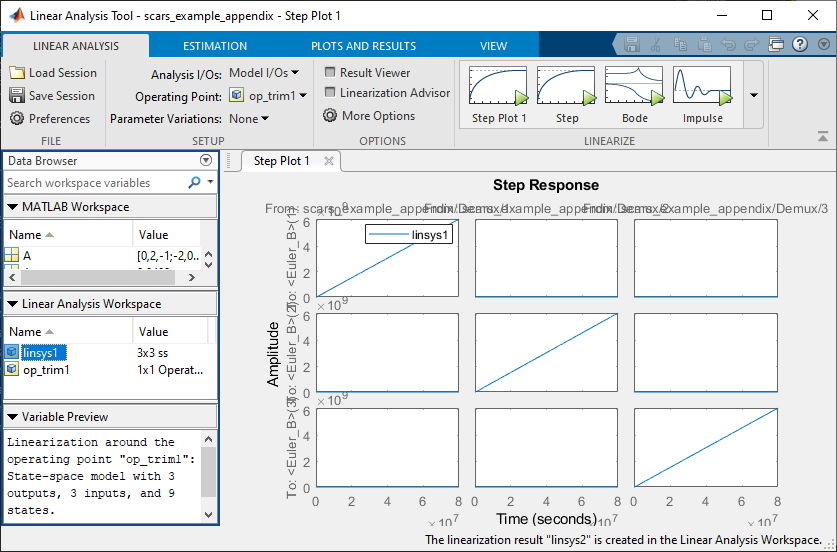
\includegraphics[width=1\textwidth]{appendix/linear.png}
            \caption{Linear Analysis Tool window after successful linearization}
            \label{fig:lin_linear}
        \end{figure}